% 2013 年春季上海卷第 16 题：f(x)=x^{-1/2} 的候选图像
% 四个小坐标系按原卷自左至右排列，依次标 (A)(B)(C)(D)。
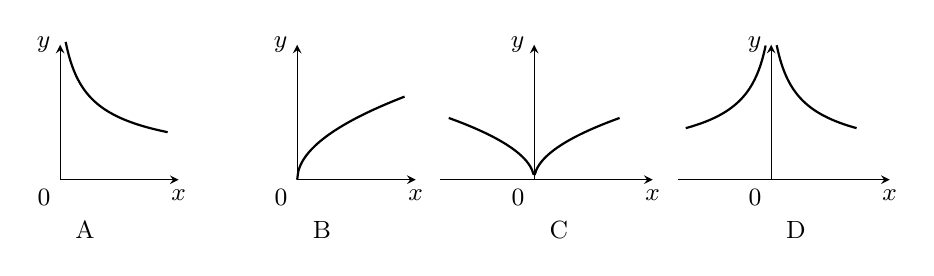
\begin{tikzpicture}[>=stealth, scale=0.70, font=\small]
  % (A) 定义域 x>0，单调递减
  \begin{scope}
    \draw[->] (0,0) -- (2.15,0) node[below] {$x$};
    \draw[->] (0,0) -- (0,2.45) node[left] {$y$};
    \node[below left] at (0,0) {$0$};
    \draw[thick, domain=0.10:1.95, samples=90, smooth]
      plot (\x,{1.25/sqrt(\x+0.15)});
    \node at (0.45,-0.92) {A};
  \end{scope}
  % (B) 过原点，单调递增
  \begin{scope}[xshift=4.30cm]
    \draw[->] (0,0) -- (2.15,0) node[below] {$x$};
    \draw[->] (0,0) -- (0,2.45) node[left] {$y$};
    \node[below left] at (0,0) {$0$};
    \draw[thick, domain=0:1.95, samples=90, smooth]
      plot (\x,{1.08*sqrt(\x)});
    \node at (0.45,-0.92) {B};
  \end{scope}
  % (C) 关于 y 轴对称，原点处取最小值
  \begin{scope}[xshift=8.60cm]
    \draw[->] (-1.70,0) -- (2.15,0) node[below] {$x$};
    \draw[->] (0,0) -- (0,2.45) node[left] {$y$};
    \node[below left] at (0,0) {$0$};
    \draw[thick, domain=-1.55:1.55, samples=120, smooth]
      plot (\x,{0.90*sqrt(abs(\x))});
    \node at (0.45,-0.92) {C};
  \end{scope}
  % (D) 关于 y 轴对称，两侧单调递减
  \begin{scope}[xshift=12.90cm]
    \draw[->] (-1.70,0) -- (2.15,0) node[below] {$x$};
    \draw[->] (0,0) -- (0,2.45) node[left] {$y$};
    \node[below left] at (0,0) {$0$};
    \draw[thick, domain=0.10:1.55, samples=90, smooth]
      plot (\x,{1.22/sqrt(\x+0.15)});
    \draw[thick, domain=-1.55:-0.10, samples=90, smooth]
      plot (\x,{1.22/sqrt(-\x+0.15)});
    \node at (0.45,-0.92) {D};
  \end{scope}
\end{tikzpicture}
